\section{OpenFace}
\label{OpenFace}
Ein Open-Source Echtzeitverfahren auf Basis von CLNF zur Bestimmung und Analyse von Gesichtsmerkmalen in Grau-Bildern und Videos. Dabei stehen für diese Anwendung nur die Kameraparameter zur Verfügung und keinerlei Zusätze wie ein Tiefenbild (kann mitverwendet werden wenn vorhanden) oder Infrarotbeleuchtung der Szene.\\
OpenFace kann 68 Landmarks ermitteln die das Gesicht beschreiben, und mit deren Hilfe Position, Blickrichtung und Gesichtsmerkmale bestimmen. Sollte ein Video als Quelle fungieren, kann OpenFace auch lernen, wodurch eine zuverlässigere Verarbeitung erzielt werden kann.\\
Als Ergebnis ist die Kopfposition (Translation und Orientierung) sowie Blickrichtung von Interesse, da mit ihnen zurückrechnet werden kann wohin die Person schaut.\\
Der Rechenaufwand zur Verarbeitung des Eingabebildes ist so ausgelegt, das ein Webcam-Video in Echtzeit ausgewertet werden kann, dies ist im aktuellen Fall nicht notwendig, da es sich um eine nachträgliche Auswertung handelt, bei der es vor allem um Genauigkeit geht.
\subsection{Bestimmung der Landmarks}
\label{bestimmung_Landmarks}
Für die Bestimmung der Landmarks wird OpenFace auf den Bildausschnitten eingesetzt. Dies bietet mehrere Vorteile, so wird nur auf Bildbereichen gearbeitet, in denen ein Gesicht zu sehen ist und unnötige Suche vermieden. Außerdem kann für jede Person die passende Initialisierung des CLNF basierend auf dem letzten Ergebnis dieser Person gewählt werden, auch für jene die nur selten dargestellt sind. Auf diese Weise kann der Bildausschnitt möglichst exakt und gleichzeitig mit den anderen ausgewertet werden.\\
Für die eigentliche Bestimmung der Landmarks bietet OpenFace zwei verschiedene Methoden, die Berechnung auf Bildern und Videos. Der Hauptunterschied ist das Lernen, dass bei der Videoauswertung verwendet wird, wodurch sich der Arbeitsbereich deutlich erhöht und bessere Ergebnisse liefert werden. Dies liegt an der Anpassung des Modells und dem möglichen Tracking der Landmarks.\\
Dies ist Interessant für die spätere Anwendung, da somit auch Einzelbilder verwendet werden können, die eine deutlich höhere Auflösung besitzen als ein Video. Allerdings sinkt bei der Verwendung von Einzelbilder der maximale Winkel relativ zur Kamera beträchtlich. Außerdem hat sich gezeigt das bei Verwendung eines Videos das Gesicht deutlich kleiner dargestellt sein kann bis keine Auswertung mehr möglich ist und sollte ein Gesicht im aktuellen Farame erfolgreichen detektiert werden auch die nachfolgenden Frames durch das lernen ausgewertet werden können.\\
Dennoch kann es passieren, dass trotz allem ein Gesicht falsch detektiert wird, wie z.B. das Erkennen eines sehr kleinen Gesichtes innerhalb einer Ohrmuschel. In solch einem Fall muss das CLNF zurückgesetzt werden, damit sich der Fehler nicht fortpflanzt.
\subsubsection{Gesichts-Landmarks: Detektion und Verfolgung}
Für die Bestimmung und Tracking der Landmarks wird ein Conditional Local Neural Fields (CLNF) eingesetzt. Dabei Handels es sich im Grunde um ein Constrained Local Model (CLM) nur mit verbesserter Patch Experts und Optimierungsfunktionen.\\
Die beiden Hauptkomponenten des CLNF von OpenFace ist das Point Distribution Model (PDM) zur Erfassung der Anordnung der Landmarks und Patch Experts zum Erfassen der Variante der einzelnen Landmarks.\\
Zu Beginn werden verschiedene initiale Hypothesen aus der dlib-Bibliothek verwendet und die Passende zur Eingabe ausgewählt. Bei den unterschiedlichen initial Hypothesen handelt es sich um die Darstellung verschiedener Gesichtsorientierungen auf denen unterschiedliche Netze trainiert wurden. Dies Herangehensweise ist langsam, aber auch exakter als eine einfache Hypothese. Wird ein Tracing, das Verfolgen der Landmarks über mehrere Frames, durchgeführt wird als initiale Hypothese das Ergebnis aus dem letzten Frame verwendet. Sollte das Tracing scheitern, wird das CNN reseted um Neu zu beginnen.\\
Auf diese Weise werden 68 Gesichts-Landmarks und  weitere 28 pro Auge erfasst. Zur Berechnung auf den Gesichtern sollten diese laut Paper \cite{OpenFace} eine Optimalgröße von 100 Pixeln für eine zuverlässige Detektion aufweisen.
\subsubsection{Detection der Gesichtsmerkmale}
Dieser Schritt kann von OpenFace ausgeführt werden, ist aber im aktuellen Fall nicht von Relevanz, da die Blickrichtung von Interesse ist und nicht die Mimik der Probanden.
\subsection{Veröffentlichte Genauigkeit}
Um die Qualität der Berechnung auf dem Kopf zu bewerten wurde der \glqq Biwi Kinect head pose\grqq \cite{BIWI_database},\glqq ICT-3DHP\grqq \cite{ICT_database} und \glqq BU Datensatz\grqq \cite{BU_database} ausgewertet. Dabei handelt es sich um Portrait-Fotos von Probanden, deren Körper in Richtung Kamera ausgerichtet ist und ihren Kopf in eine beliebige Richtung drehen. Für die Genauigkeit der Kopfposition haben sich folgend Werte ergeben in Grad:\\
\begin{tabular}{|l|c|c|c||c|c|}
	\hline
	&Yaw&Pitch&Roll&Mean&Median\\\hline
	Biwi Kinect&7.9&5.6&4.5&6.0&2.6\\\hline
	BU dataset&2.8&3.3&2.3&2.8&2.0\\\hline
	ICT-3DHP&3.6&3.6&3.6&3.6&-\\\hline
\end{tabular}\\\\
Für die Qualität wurde der Augendatensatz \glqq Appearancebased
gaze estimation in the wild\grqq \cite{database_Eye_old} zur Bestimmung der Blickrichtung verwendet und es ergab sich ein durchschnittlichen Fehler von 9.96 Grad.
\subsection{Auswirkung der Größe}
Durch die Aufgabenstellung muss das Verfahren zuverlässig bezüglich der Distanzen bzw. Darstellungsgröße sein. Zur Messung wurde der Datensatz von Labeled Faces in the Wild \cite{database_Face} verwendet. In diesem Datensatz ergibt sich im Originalbild eine durchschnittliche Kopfbreite von 94 Pixel. Bei Random Forests for Real Time 3D Face Analysis \cite{database_Face_Ori} ist die durchschnittliche Breite 78 Pixel.\\
Zur Durchführung wurden die Größe der Bilder mit dem Skalierungsfaktor multipliziert und linear verkleinert um so kleinere, weiter entferntere Gesichter zu erhalten und anschließend mit dem Image-Detector von OpenFace zu verarbeiten. Das Ergebnis ist in \autoref{img_lineareverkleinerung} dargestellt.\\
Es ist zu erkennen, dass die Wahrscheinlichkeit auf eine erfolgreiche Detektion ab $0.5$, also Gesichert mit etwa 47 Pixel Breite, rapide abnimmt. Bei der in \autoref{hardware} beschriebenen Kamera entspricht dies einer Distanz von etwa $4.5m$.\\
Bei der maximalen Distanz auf der gearbeitet werden soll $(8.5m)$ ergibt sich eine Gesichtsgröße von etwa 22 Pixel, das einer Skalierung von 0.25 entspricht. Bei dieser Bildgröße ist in der Standardanwendung ohne Skalierung keine Detektion möglich, siehe \autoref{img_lineareverkleinerung}.
\begin{figure}
	\centering
	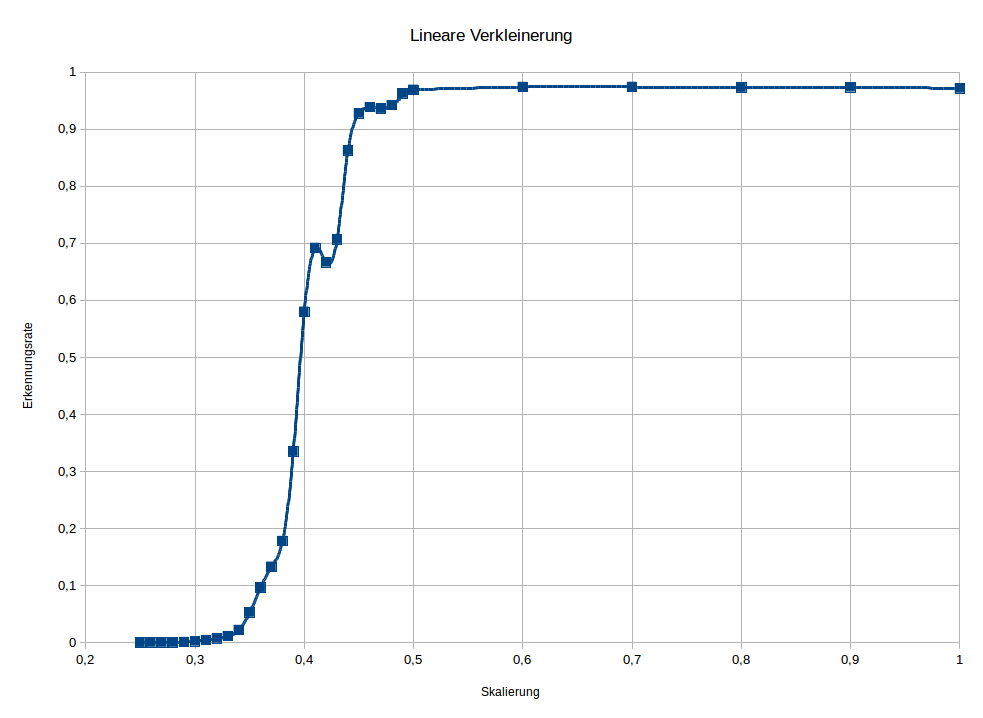
\includegraphics[width=0.45\linewidth]{img/lineare_Verkleinerung}
	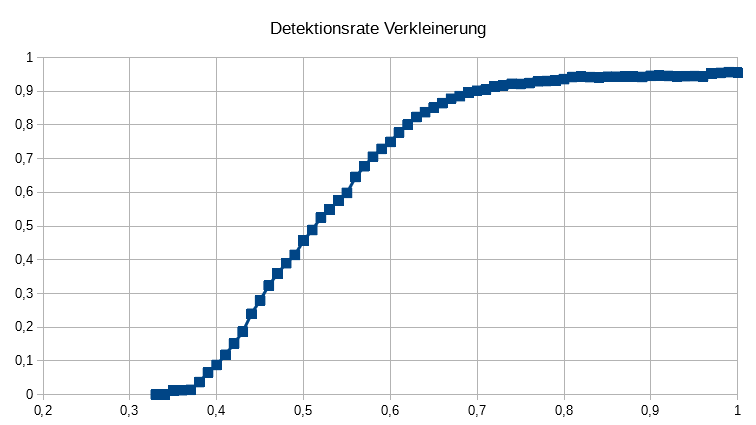
\includegraphics[width=0.45\linewidth]{img/lineare_Verkleinerung2}
	\caption{Die Bilder aus Labeled Faces in the Wild \cite{database_Face} (links) und Random Forests \cite{database_Face_Ori} wurden mit den Faktor auf der X-Achse linear verkleinert und die Erkennungsrate Y-Achse abgebildet}
	\label{img_lineareverkleinerung}
\end{figure}
\subsection{Auswirkung der verschiedenen Skalierungesverfahren auf Detektion}
\label{OpenFace_skal}
Um auf den gewünschten Distanzen arbeiten zu können, wird der jeweilige Bereich hochskaliert. Dazu wird das Ursprüngliche Bild $(250\times 250)$ linear um den angegebene Faktor verkleinert und anschließend mit den angegebenen Verfahren auf $300\times 300$ wieder vergrößert, damit die abgebildeten Gesichter in etwa 100 Pixel groß sind. Die Wahrscheinlichkeit auf eine Detektion ist in \autoref{img_hochskalliern} dargestellt.\\
Es ist zu erkennen das durch die Vergrößerung, jene Gesichter in Bereichen die normal nicht erkennbar sind, ausgewertet werden können.\\
Als das ungeeignetste Verfahren hat sich Nearest-Neighbor herausgestellt, siehe blaue Linie \autoref{img_hochskalliern}, da die Detektionsrate deutlich früher abfällt als bei den anderen. Die anderen haben sehr ähnliche Ergebnisse, nur das Lineare Verfahren ist etwas schlechter. Dennoch werden die Anforderungen, eine Detektion auf Gesichtern mit 22 Pixel (Skalierung 0.25), von allen erfüllt.\\
Ausgehend vom Skalierungsfaktor des Linearen-, Bicubic- und Lanczos-Verfahren wären mit der verwendeten Kamera auch Distanzen bis zu $14m$ möglich. Allerdings ist das Bild durch die Verkleinerung  deutlich besser als Originalaufnahmen, da Pixelrauschen und Ähnliches nicht vorhanden ist.
\begin{figure}
	\centering
	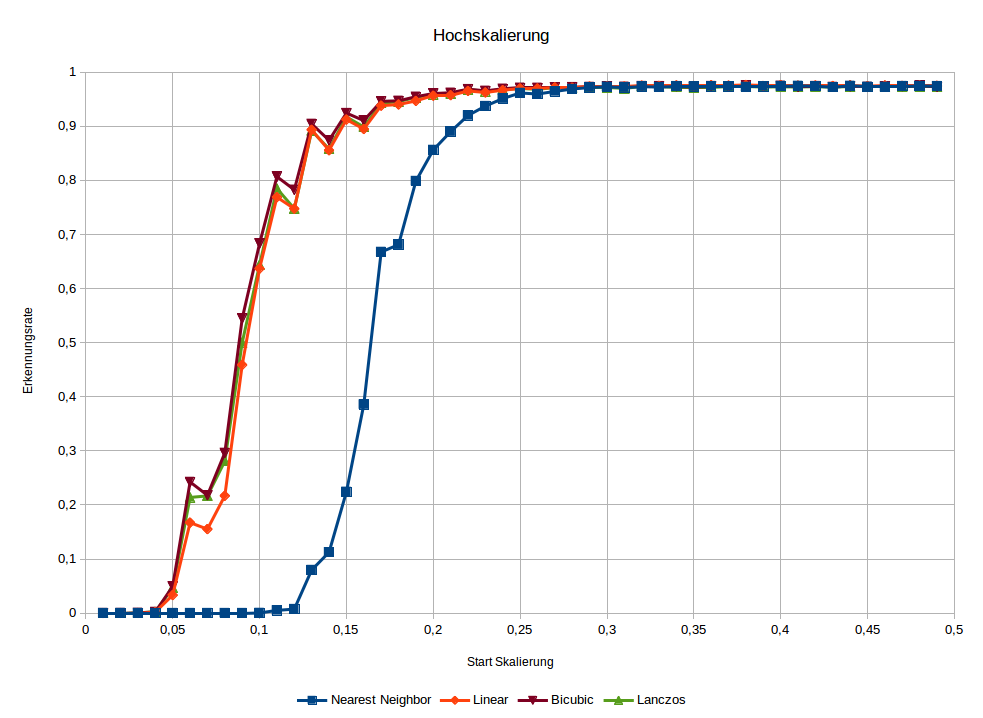
\includegraphics[width=0.5\linewidth]{img/Hochskalliern}
	\caption{Die Bilder aus Labeled Faces in the Wild \cite{database_Face} wurden mit den Faktor auf der X-Achse linear verkleinert und mit den verschiedenen Verfahren wieder vergrößert \autoref{scale_Algos}. Aufgetragen gegen die Detektionswahrscheinlichkeit.
		Nearest-Neighbor (blau), Linear (rot), Bicubic (braun), Lanczos (grün)}
	\label{img_hochskalliern}
\end{figure}
\subsection{Auswirkung von Pixelrauschen auf Detektion}
Mit diesem Test soll geprüft werden, welches der Verfahren auch stabil gegen Rauschen ist.\\
Um Pixelrauchen zu simulieren, wurden die Bilder aus Labeled Faces in the Wild \cite{database_Face} entsprechend verkleinert, mit Rauschen versehen um sie anschließend mit den unterschiedlichen Verfahren zu vergrößern.\\
Das Rauschen wird für jedes Pixel simuliert, indem eine Wahrscheinlichkeit von $50\%$ besteht, eine gleich verteilte Abweichung von $\pm 10\%$ des Originalen Farbwertes. Dieser Vorgag wurde für jedes Bild viermal wiederholt um Zufälligkeiten bei der Rauschsimulation zu vermeiden.\\
Wie zu erwarten ist Nearest-Neighbor am schlechtesten, aber auch zwischen den anderen Verfahren sind nun unterscheiden zu erkennen, siehe \autoref{img_hochskalliern_nois}. Die gesamte Erkrankungsrate ist signifikant kleiner als ohne Rauschen, wobei die Position $(0.15)$, ab welcher die Erkennungsrate rapide abfällt, beibehalten wird.
\begin{figure}
	\centering
	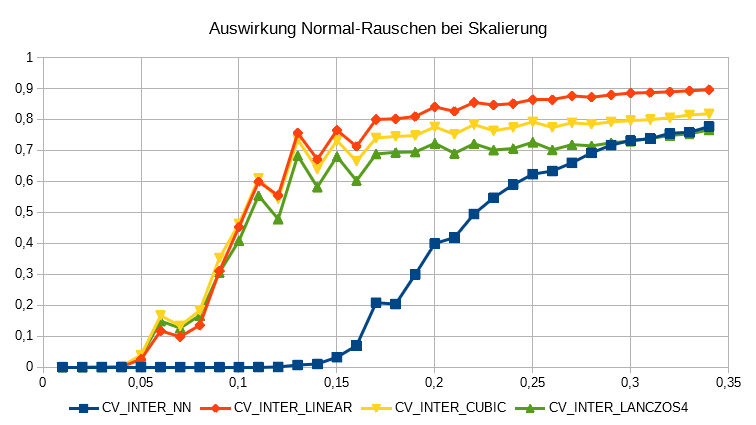
\includegraphics[width=0.7\linewidth]{img/Hochskalliern_Nois}
	\caption{Bilder aus Labeled Faces in the Wild \cite{database_Face}, mit dem X-Faktor verkleinert, um jedes Pixel mit $50\%$ Wahrscheinlichkeit auf $\pm 10\%$ Gleichverteilung der Abweichung}
	\label{img_hochskalliern_nois}
\end{figure}
\subsection{Arbeitsbereich bezüglich Rotation}
Von Interesse sind auch die Winkel, bei den Gesichter in verschiedenen Skalierungen noch erkannt werden, siehe \autoref{img_Rot_Value}.\\
Hier ist zu erkennend das der Wertebereich ab 0.7 abnimmt und ab 0.5 recht schnell. Dieser Bereich ist von Interesse, da selbst wenn ein Gesicht in dieser Größe allerdings außerhalb des Wertebereiches vorhanden sein sollte, dieses nicht erkannt wird.\\
Der Wertebereich auf den einzelnen Achsen ist ausreichend für die Anwendung sollte das Ziel der Aufmerksamkeit sich in der näher der Kamera befinden. Auch wenn die Rotation parallel zur Horizontalen etwas größer sein könnte.
\begin{figure}
	\centering
	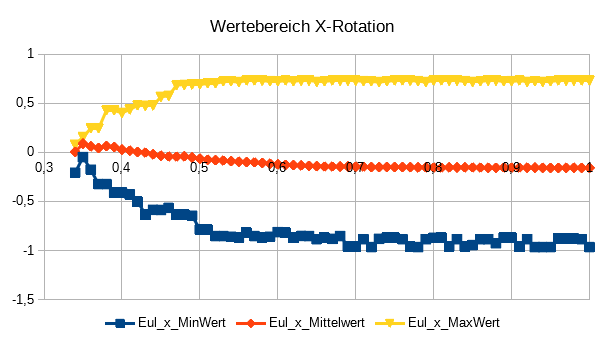
\includegraphics[width=0.3\linewidth]{tabelle/X_Rot}
	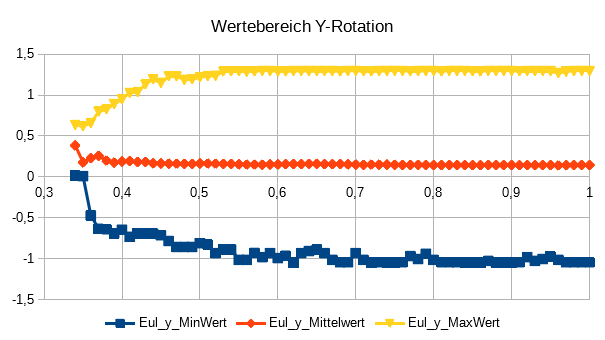
\includegraphics[width=0.3\linewidth]{tabelle/Y_Rot}
	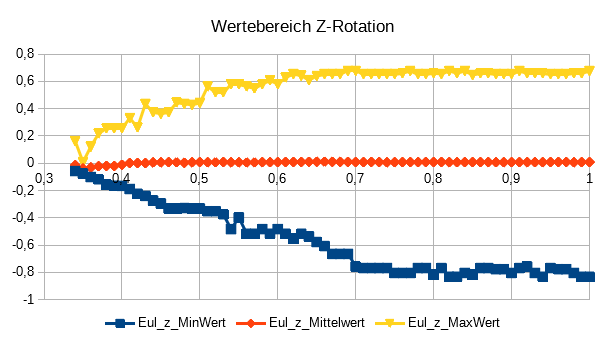
\includegraphics[width=0.3\linewidth]{tabelle/Z_Rot}
	\caption{Darstellung der noch detektierten Wertebereiche in Bogenmaß.}
	\label{img_Rot_Value}
\end{figure}